% === INTRO === %

\vspace{1em}
\subsection{Introducción teórica} Ya vimos que si los autovalores son todos diferentes en módulo el método funciona bien. 
¿Qué es lo que pasa cuando hay autovalores de igual módulo?


\vspace{2em}
\noindent \textsc{Método de la potencia para autovalores dominantes repetidos}

\vspace{2em}
\noindent Para simplificar el analisis separamos en casos: \\
\indent 1) 2 autovalores dominantes que son iguales \\
\indent 2) 2 autovalores dominantes que tienen el mismo valor absoluto pero son diferentes
\vspace{2em}



\noindent \textsc{1) Método de la potencia para autovalores dominantes iguales}
\begin{align}
    let \ norm \ :&= \ ||\sum_{i=1}^{n} a_i \ * \ \lambda_{i}^{k} \ * \ x_i||_2 \\
    \lim_{k \to \infty} y_k &= \frac{\sum_{i=1}^{n} a_i * \lambda_{i}^{k} * x_i }{norm} \\ 
    \lim_{k \to \infty} y_k &= \frac{(\sum_{i=1}^{n} a_i * \lambda_{i}^{k} * x_i) / \lambda_{1}^{k}}{norm / \lambda_{1}^{k}} \\
    let \ b_i \ :&= \ sign(\lambda_{1}^{k}) * \frac{a_i}{norm / |\lambda_{1}^{k}|} \\
    \lim_{k \to \infty} y_k &= \sum_{i=1}^{n} b_i * \frac{\lambda_{i}^{k}}{\lambda_{1}^{k}} * x_i \\
    \lim_{k \to \infty} y_k &= b_1 * x_1 + b_2 * x_2 
\end{align}

\vspace{1em}
Pero algo interesante es que como $x_1$ y $x_2$ son autovectores con el mismo $\lambda$ entonces:
\begin{align}
    dados\ c_1 \ y \ c_2 &\in \mathbb{R} \\
    A * (c_1 * x_1 + c_2 * x_2) &= A * c_1 * x_1 + A * c_2 * x_2 \\
    A * (c_1 * x_1 + c_2 * x_2) &= \lambda * c_1 * x_1 + \lambda * c_2 * x_2 \\
    A * (c_1 * x_1 + c_2 * x_2) &= \lambda * (c_1 * x_1 + c_2 * x_2) 
\end{align}

Lo que se puede concluir de este resultado es que no importa quienes sean $c_1$, $c_2$ se cumple que ($c_1 * x_1 + c_2 * x_2$) es un autovector y $\lambda$ es su autovalor por lo tanto en el caso donde hay 2 autovalores dominantes iguales, el metodo de la potencia converge correctamente, además vale no solo cuando la cantidad de autovalores dominantes repetidos son 2 sino que no importa la cantidad de veces que esté repetido el autovalor dominante se cumple que $\sum_{i=1}^{n} (a_i \ * \ \lambda_{i}^{k} \ * \ x_i)$ resulta en un autovector de A

\vspace{1em}

Cabe destacar que como $(c_1 * x_1 + c_2 * x_2)$ es autovector $\forall c_1, c_2$ es lo mismo que decir que cualquier combinación lineal de $x_1$ y $x_2$ va a ser autovector por ende hay infinitas posibilidades para los 2 autovectores dominantes. A diferencia del caso en el que todos los autovalores son diferentes en módulo donde solo hay dos autovectores con norma 2 igual a 1, ahora las posibilidades son infinitas, por lo tanto hay que tener esto en mente a la hora de realizar comparaciones con los resultados que obtiene numpy. 

\vspace{1em}

Algo interesante es que si $\lambda$ es negativo el método oscila entre iteraciones pares e iteraciones impares convergiendo a 2 vectores diferentes. $b_i$ esta definido de la siguiente manera: $sign(\lambda^{k}) * \frac{a_i}{norm / |\lambda^{k}|}$, si llamamos $d_i$ a $\frac{a_i}{norm / |\lambda^{k}|}$ entonces en las iteraciones pares $sign(\lambda^{k}) = 1$ por lo tanto, $\lim_{k \to \infty} y_k = (d_1 * x_1 + d_2 * x_2)$ pero en las impares $sign(\lambda^{k}) = -1$ por lo tanto, $\lim_{k \to \infty} y_k = -(d_1 * x_1 + d_2 * x_2)$, ambos son autovectores válidos pero el método depende de la distancia entre una iteración y su consecutiva, como en este caso el método oscila entre iteraciones pares e iteraciones impares la distancia entre una iteración y su consecutiva no tiende a 0, por lo que el método va a tener que que hacer el total de las iteraciones sin poder interrumpirse. De esta observación concluimos que es conveniente hacer el método de la potencia de a 2 pasos por vez, pero debería converger correctamente a un autovector sin ninguna modificación.


\noindent \textsc{2) Método de la potencia para autovalores diferentes pero iguales en módulo}
\begin{align}
    let \ norm \ :&= \ ||\sum_{i=1}^{n} a_i \ * \ \lambda_{i}^{k} \ * \ x_i||_2 \\
    \lim_{k \to \infty} y_k &= \frac{\sum_{i=1}^{n} a_i * \lambda_{i}^{k} * x_i }{norm} \\ 
    \lim_{k \to \infty} y_k &= \frac{(\sum_{i=1}^{n} a_i * \lambda_{i}^{k} * x_i) / \lambda_{1}^{k}}{norm / \lambda_{1}^{k}} \\
    let \ b_i \ :&= \ \frac{a_i}{norm / \lambda_{1}^{k}} \\
    \lim_{k \to \infty} y_k &= \sum_{i=1}^{n} b_i * \frac{\lambda_{i}^{k}}{\lambda_{1}^{k}} * x_i \\
    \lim_{k \to \infty} y_k &= b_1 * x_1 + b_2 * \frac{\lambda_{2}^{k}}{\lambda_{1}^{k}} * x_2 \\
    \lim_{k \to \infty} y_k &= b_1 * x_1 + b_2 * sign(\lambda_{2}^{k}) * x_2 
\end{align}

\vspace{1em}

\noindent Notamos que este vector también oscila entre k par y k impar, ya que si k es par: \\
\indent\indent $\lim_{k \to \infty} y_k = b_1 * x_1 + b_2 * x_2$ \\ \\
Pero si k es impar: \\
\indent \indent $\lim_{k \to \infty} y_k = b_1 * x_1 - b_2 * x_2$ \\ \\
Se ve claramente que si $b_2 * x_2$ no es 0 son dos vectores diferentes.
Pero para mayor seguridad lo comprobamos experimentalmente, como se puede observar en el siguiente gráfico:

\vspace{1em}
\begin{figure}[!htbp]
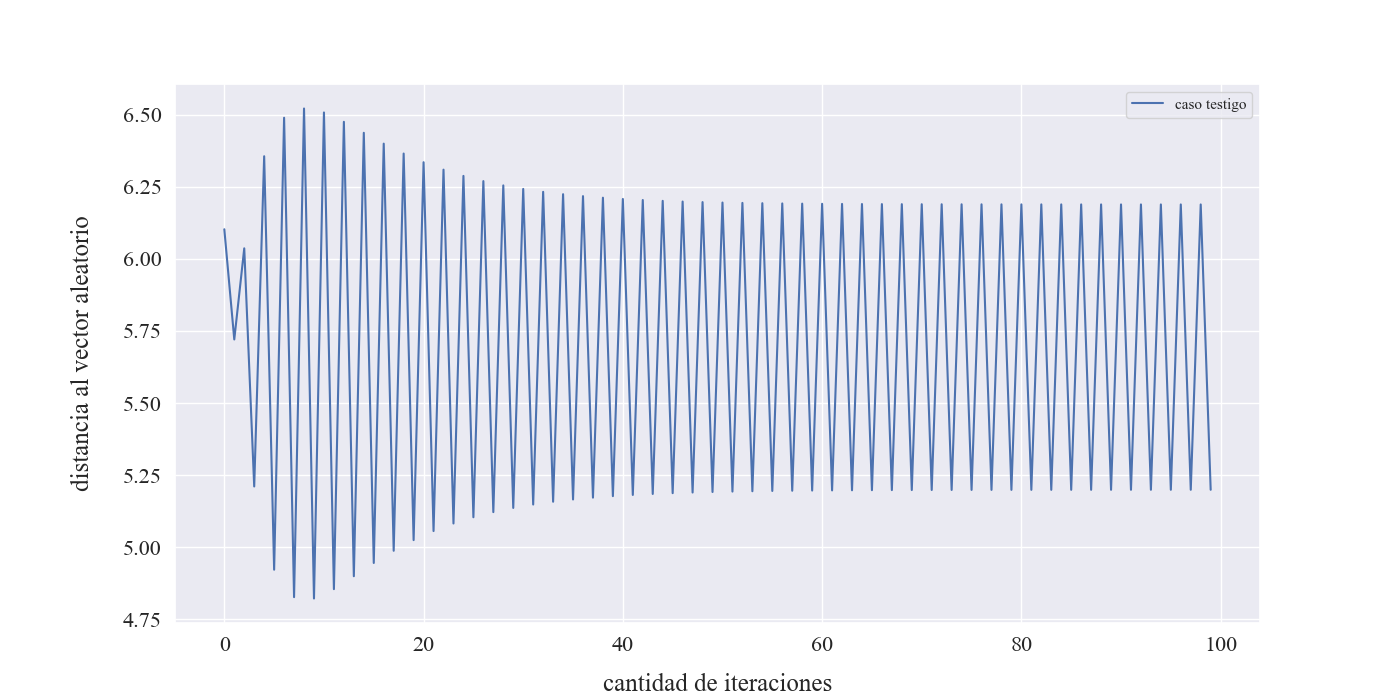
\includegraphics[scale=0.55, trim=100 80 100 100, clip]{files/src/.media/op_oscilante.png}
\caption{Se eligió un vector aleatorio constante normalizado y en cada iteración del metodo de la potencia calculamos $||randVector - y_k||_2$. Se puede apreciar claramente como la distancia al randVector oscila entre las iteraciones pares e impares.}
\end{figure}


\vspace{1em}

Queremos ver si alguno de los vectores a los que converge $y_k$ es autovector de A:
\begin{align}
    dados\ c_1 \ y \ c_2 &\in \mathbb{R} \\
    A * (c_1 * x_1 + c_2 * x_2) &= A * c_1 * x_1 + A * c_2 * x_2 \\
    A * (c_1 * x_1 + c_2 * x_2) &= \lambda * c_1 * x_1 - \lambda * c_2 * x_2 \\
    A * (c_1 * x_1 + c_2 * x_2) &= \lambda * (c_1 * x_1 - c_2 * x_2) 
\end{align}

Lo que se puede concluir de este resultado es que si $c_1$ y $c_2$ son ambos desiguales a 0 entonces $(c_1 * x_1 + c_2 * x_2)$ no es autovector. Teniendo en cuenta que $b_i \ := \ \frac{a_i}{norm / \lambda_{1}^{k}}$ y $a_1$, $a_2$ pueden no ser 0, por lo tanto podemos afirmar con seguridad que si hay un autovalor positivo y un autovalor negativo dominantes con el mismo módulo, entonces $\lim_{k \to \infty} y_k = b_1 * x_1 + b_2 * sign(\lambda_{2}^{k}) * x_2$ que por lo mencionado previamente NO es autovector de la matriz inicial.

\vspace{1em}

Con este resultado en mente observamos que en caso de computar la suma entre las últimas dos iteraciones del método de la potencia obtendríamos lo siguiente:

\vspace{1em}
Dado k par suficientemente grande para que el método converja: 
\begin{align}
    y_k &= b_1 * x_1 + b_2 * x_2 \\ 
    y_{k+1} &= b_1 * x_1 - b_2 * x_2 \\ 
    y_k + y_{k+1} &= b_1 * x_1 + b_2 * x_2 + b_1 * x_1 - b_2 * x_2 \\ 
    y_k + y_{k+1} &= 2 * b_1 * x_1
\end{align}

Sabemos que $x_1$ es autovector, por ende $2 * b_1 * x_1$ también es autovector.
Observamos que se podría calcular la resta para obtener el otro autovector($x_2$) pero la deflacíon asume que el método de la potencia encuentra de a 1 autovector por llamado por lo que habría que cambiar varios algoritmos para poder aprovechar este caso puntual y consideramos que no vale la pena.

\vspace{1em}
Con este resultado en mente planteamos una alternativa al método de la potencia de la siguiente forma:


